\documentclass{beamer}

%Packages
\usepackage[utf8]{inputenc}
\usepackage{hyperref}

%META-INFORMATION
\title{Semantic Search for Quantity Expressions}
\author{Tom Wiesing\\\ \\Supervisor: Michael Kohlhase\\Co-supervisor: Tobias Preusser}
\date{May 20, 2015 \\110392 Guided Research Applied and Computational Mathematics \& Thesis}

\begin{document}
  %TITLEPAGE
  \frame{\titlepage}

  %OVERVIEW
  \begin{frame}{Overview}
    \pause
    \begin{columns}[T]
      \begin{column}[T]{7cm}
        \begin{itemize}[<+->]
          \item Motivation: Problem and State Of The Art
          \item Our Approach: Structure Of The Search Engine
          \item The Implementation
          \item Time for Questions
        \end{itemize}
      \end{column}
    \end{columns}
  \end{frame}

  %MOTIVATION
  \begin{frame}{Motivation (1)}
    \begin{itemize}[<+->]
      \item We use units every day
      \item We encounter them everywhere:
      \begin{itemize}[<+->]
        \item When driving, there are speed limits, for example: \raisebox{-0.5\height}{
\includegraphics[width=10mm]{imgs/sign60.png}} $\frac{\text{km}}{\text{h}}$ % http://www.gettingaroundgermany.info/g_imgs/z274.gif
        \item When baking, it often says in recepies something like: ``add 3 tea spoons of sugar''
        \item When shopping for shoes there are different sizes
      \end{itemize}
      \item In scientific papers they occur a lot
      \item everything which somehow models a real system has at least one quantity expression
      \item everything is quantified
    \end{itemize}
  \end{frame}

  \begin{frame}{Motivation (2)}
    \begin{itemize}[<+->]
      \item But where is the problem?
      \item Within one paper only a handful of units is used
      \item In general there are \textbf{a lot} of \textbf{different} units to describe \textbf{the same} quantity
      \item Just for lengths: \pause \textit{Meter}, \pause \textit{Inch}, \pause \textit{Foot}, \pause \textit{Mile}, \pause \textit{Nautical Mile}, \pause $\dots$
      \item This can cause problems when not converting properly
      \item Mars Climate Orbiter (1999) \\ 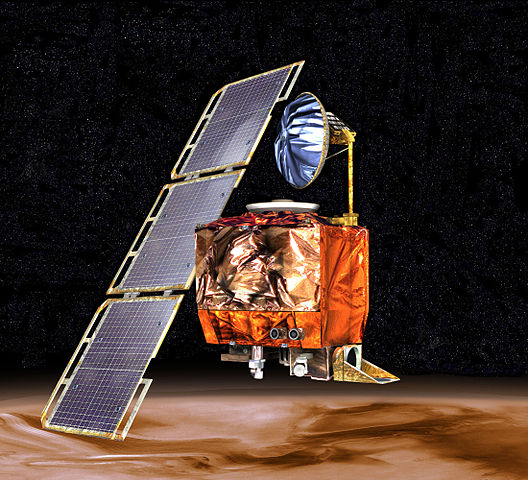
\includegraphics[width=50mm]{imgs/mco.jpg}
      % http://upload.wikimedia.org/wikipedia/commons/thumb/1/19/Mars_Climate_Orbiter_2.jpg/528px-Mars_Climate_Orbiter_2.jpg
      \item Different Units are a big problem
    \end{itemize}
  \end{frame}

  \begin{frame}{Motivation (3)}
    \pause
    \begin{itemize}[<+->]
      \item What is the most common solution?
      \item Unit Converters
      \begin{itemize}[<+->]
        \item There are a lot of these \\ 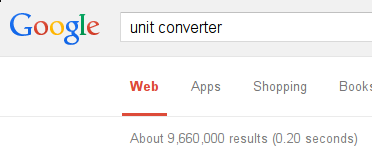
\includegraphics[width=40mm]{imgs/google.png}
        \item Google itself has one integrated \\ 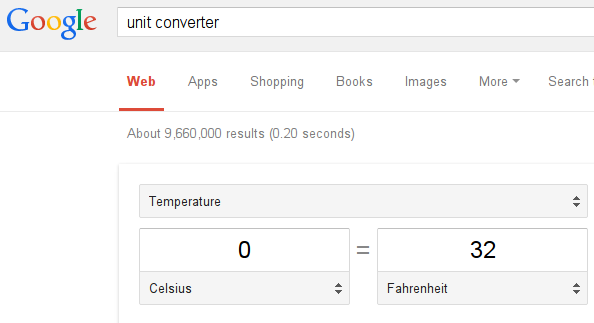
\includegraphics[width=40mm]{imgs/googleuc.png}
      \end{itemize}
    \end{itemize}
  \end{frame}

  \begin{frame}{Motivation (4)}
    \begin{itemize}[<+->]
      \item user needs to find out that conversion is required
      \item both input \textbf{and} output units need to be \textbf{given}
      \item this is not integrated into the search process itself
      \item Wouldn't it be nice:
      \begin{itemize}[<+->]
        \item when searching for $25\ \frac{\text{m}}{\text{s}}$
        \item we also find $90\ \frac{\text{km}}{\text{h}}$
        \item we did not have to search for all the representations of the same quantity expression
      \end{itemize}
      \item This is the kind of search engine we have built
    \end{itemize}
  \end{frame}

  \begin{frame}{Our Approach (1)}
    \begin{itemize}[<+->]
      \item What components do we need for a semantic search engine?
      \begin{enumerate}[<+->]
        \item A \textit{Unit System} that is aware of the different representations of a QE
        \item A \textit{Spotter} that finds representations of QEs inside documents
        \item A \textit{Search Algorithm} that given a QE finds all its representations in the system
        \item A \textit{Frontend} that allows queries to be made
      \end{enumerate}

      \item Spotter is done by \textit{Stiv Sherko}
      \item We only need to worry about the \textit{Unit System}, the \textit{Search Algorithm} and the \textit{Frontend}
    \end{itemize}
  \end{frame}

  \begin{frame}{Our Approach: The Unit System (1)}
    \begin{itemize}[<+->]
      \item Let's start with the Unit System
      \item We orient ourselves on the SI specification
      \item Each quantity has a dimension
      \item According to SI there are 7 basic ones:
      \begin{itemize}
        \item length
        \item mass
        \item time
        \item electric current
        \item temperature
        \item luminous intensity
        \item amount of substance
      \end{itemize}
      \item but there are also quantities where we just \textit{count}
      \item and \textit{dimensionless quantities} (such as Information)
      \item so we have 9 basic dimensions
    \end{itemize}
  \end{frame}

  \begin{frame}{Our Approach: The Unit System (2)}
    \begin{itemize}[<+->]
      \item we can also multiply these to get new dimensions
      \item such as area $=$ length $\cdot{}$ length
      \item similarly we can divide dimensions
      \item We can use this to get a meta-mathematical formalisation of dimensions
    \end{itemize}
  \end{frame}
  \begin{frame}{Our Approach: The Unit System (3)}
      \begin{center}
        \begin{tabular}{|l c l|}
          \hline
          \textsf{Dimension} & &\\\hline
          $\mathsf{dimension}$ & $:$ & $ \mathsf{type}$\\

          $\mathsf{none}$ & $:$ & $ \mathsf{dimension}$\\
          $\mathsf{count}$ & $:$ & $ \mathsf{dimension}$\\
          $\mathsf{length}$ & $:$ & $ \mathsf{dimension}$\\
          $\mathsf{mass}$ & $:$ & $ \mathsf{dimension}$\\
          $\mathsf{time}$ & $:$ & $ \mathsf{dimension}$\\
          $\mathsf{current}$ & $:$ & $ \mathsf{dimension}$\\
          $\mathsf{temperature}$ & $:$ & $ \mathsf{dimension}$\\
          $\mathsf{luminous}$ & $:$ & $ \mathsf{dimension}$\\
          $\mathsf{amount}$ & $:$ & $ \mathsf{dimension}$\\

          $\cdot{}$ & $:$ & $ \mathsf{dimension} \rightarrow \mathsf{dimension} \rightarrow \mathsf{dimension}$\\
          $\backslash$ & $:$ & $ \mathsf{dimension} \rightarrow \mathsf{dimension} \rightarrow \mathsf{dimension}$\\\hline
        \end{tabular}
    \end{center}
  \end{frame}



  % \begin{frame}{Carl David Tolmé Runge - The end (2)}
  %     \begin{itemize}
  %         \item Sources:
  %         \begin{itemize}
  %             \item \url{http://en.wikipedia.org/w/index.php?title=Carl_David_Tolm\%C3\%A9_Runge}
  %             \item \url{http://de.wikipedia.org/w/index.php?title=Carl_Runge}
  %             \item \url{http://www-history.mcs.st-and.ac.uk/Mathematicians/Runge.html}
  %             \item \url{http://en.wikipedia.org/wiki/Runge\%E2\%80\%93Kutta_methods}
  %             \item \url{http://en.wikipedia.org/wiki/List_of_Runge\%E2\%80\%93Kutta_methods}
  %         \end{itemize}
  %         \item Image sources:
  %         \begin{itemize}
  %             \item \url{http://upload.wikimedia.org/wikipedia/commons/3/34/CarleRunge.jpg}
  %             \item \url{http://www-rohan.sdsu.edu/\~jmahaffy/courses/f00/math122/lectures/num_method_diff_equations/images/euler_ani.gif}
  %         \end{itemize}
  %     \end{itemize}
  % \end{frame}

\end{document}
